\subsection{Dyna-Q in Modern Notation}
\label{section:fc_dyna_q}

Dyna-Q combines tabular $Q$-learning with a learned one-step model and applies $K$ planning updates after each real interaction.

\subsubsection{Algorithm}
\label{section:fc_dyna_q_algorithm}

The setting is a finite Markov decision process with state space $\mathcal{S}$ and action space $\mathcal{A}$. The agent maintains a tabular action-value function $Q : \mathcal{S} \times \mathcal{A} \to \mathbb{R}$, a learned transition model $\widehat P(s' \mid s, a)$, and a learned reward model $\widehat r(s, a)$. The parameters are a step size $\alpha \in (0, 1]$, a discount factor $\gamma \in [0, 1)$, an exploration parameter $\varepsilon \in (0, 1)$, and a planning-step count $K \in \mathbb{N}$. The agent initializes $Q$, $\widehat P$, and $\widehat r$ to arbitrary values.

For each step $t$:
\begin{enumerate}
  \item Observe the current state $s$ and select an action $a \in \arg\max_{a'} Q(s, a')$ with $\varepsilon$-greedy exploration, breaking ties uniformly at random.
  \item Execute $a$ in the environment and observe the reward $r$ and the next state $s'$.
  \item Direct RL update,
        \[ Q(s, a) \leftarrow Q(s, a) + \alpha \big[ r + \gamma \max_{a''} Q(s', a'') - Q(s, a) \big]. \]
  \item Model update, $\widehat r(s, a) \leftarrow r$ and $\widehat P(\cdot \mid s, a) \leftarrow \delta_{s'}$, recording the most recent observed transition as a deterministic prediction.
  \item Planning. Repeat $K$ times, on each iteration sampling a previously-visited pair $(\tilde s, \tilde a)$ uniformly from the agent's experience, querying $\widehat r(\tilde s, \tilde a)$ and $\widehat P(\cdot \mid \tilde s, \tilde a)$ to obtain a synthetic transition $(\tilde r, \tilde s')$, and applying the same $Q$-update as in step 3,
        \[ Q(\tilde s, \tilde a) \leftarrow Q(\tilde s, \tilde a) + \alpha \big[ \tilde r + \gamma \max_{a''} Q(\tilde s', a'') - Q(\tilde s, \tilde a) \big]. \]
\end{enumerate}

Step 3 is the tabular $Q$-learning update of \citet{WatkinsDayan1992}. Under the standard step-size and visitation conditions, it converges to $Q^\star$ by the $\gamma$-contraction of the Bellman optimality operator (Theorems~\ref{thm:qlearning_convergence} and~\ref{thm:q_factor_contraction}, Section~\ref{sec:planning_learning}). Step 5 applies the same update to rewards and transitions generated by $\widehat r$ and $\widehat P$. For a fixed tabular model, the planning updates converge to the model's optimal action values under the corresponding step-size and visitation conditions. Convergence to the environment's $Q^\star$ additionally requires the learned model to become accurate on the state-action pairs used for planning. With function approximation, Lipschitz bounds provide one way to relate errors in the learned model to errors in the resulting value function (\citealt{Asadi2018Lipschitz}; \S\ref{section:fc_synthesis_fails}).

Steps 3 and 5 use the same $Q$-learning update. Step 3 uses a transition observed through interaction with the environment. Step 5 samples a previously visited state-action pair and obtains the reward and successor state from the learned model. Dyna-Q therefore plans by applying the learning rule to model-generated experience. The value of $K$ sets the number of model-generated updates per observed transition.

\subsubsection{Dyna Maze Experiment}
\label{section:fc_dyna_q_empirics}

\citet{sutton2018} compare planning-step counts $K \in \{0, 5, 50\}$ in a deterministic sparse-reward gridworld. With $K = 0$, the planning loop is omitted and the method reduces to plain $Q$-learning. Near-optimal performance requires roughly three episodes with $K = 50$ and roughly twenty-five with $K = 0$. The reduction in environment interactions comes with fifty model-based updates per real step and depends on sufficiently accurate model predictions. In the blocking-maze variant, an exploration bonus helps the agent adapt after the transition structure changes.

\subsubsection{Model Choice and Simulated Updates}
\label{section:fc_dyna_q_architecture}

Dyna does not prescribe a model class. The algorithm above uses a deterministic one-step Dirac model $\widehat P(\cdot \mid s, a) \leftarrow \delta_{s'}$, but the generic architecture also permits probabilistic and imperfect learned models. Later methods make different choices. \citet{HaSchmidhuber2018} use a convolutional variational autoencoder paired with a mixture-density recurrent network (\S\ref{section:fc_ha_schmidhuber}). PlaNet and Dreamer use a Recurrent State-Space Model that couples a deterministic recurrent path with a stochastic latent (\S\ref{section:fc_rssm}). MuZero omits observation reconstruction and trains its model against quantities used in value calculation (\S\ref{section:fc_value_aware}). MBPO uses a deep ensemble of probabilistic feed-forward networks (\S\ref{section:fc_mbpo}).

Dyna-Q applies the same Bellman update to real and simulated transitions. Direct methods update values from interaction, whereas indirect methods use a model for planning. Dyna-Q processes both sources with $Q$-learning, and $K$ determines how many model-generated updates follow each observed transition. Later model-based methods also use learned models to improve policies or values, although their inner loops may use tabular updates, fitted $Q$-iteration, soft actor-critic, or model predictive control. In economic terms, Dyna augments adaptive learning with simulated experience between observations. Its effect on sample efficiency depends on whether the learned model is accurate enough for the planner's decisions.

\subsubsection{Simulation Study: Planning Amplification in the Blocking Maze}
\label{section:fc_dyna_q_sim}

The simulation measures cumulative reward under a common environment-step budget. Following \citet{sutton2018}, it compares Dyna-Q across different numbers of planning updates. Plain $Q$-learning provides a no-planning comparison in the sparse-reward maze. After environment step $t = 1000$, the wall opening changes location and previously recorded transition predictions can become stale. Figure~\ref{figure:fc_dyna_maze_layout} shows the two maze layouts.

\begin{figure}[ht]
  \centering
  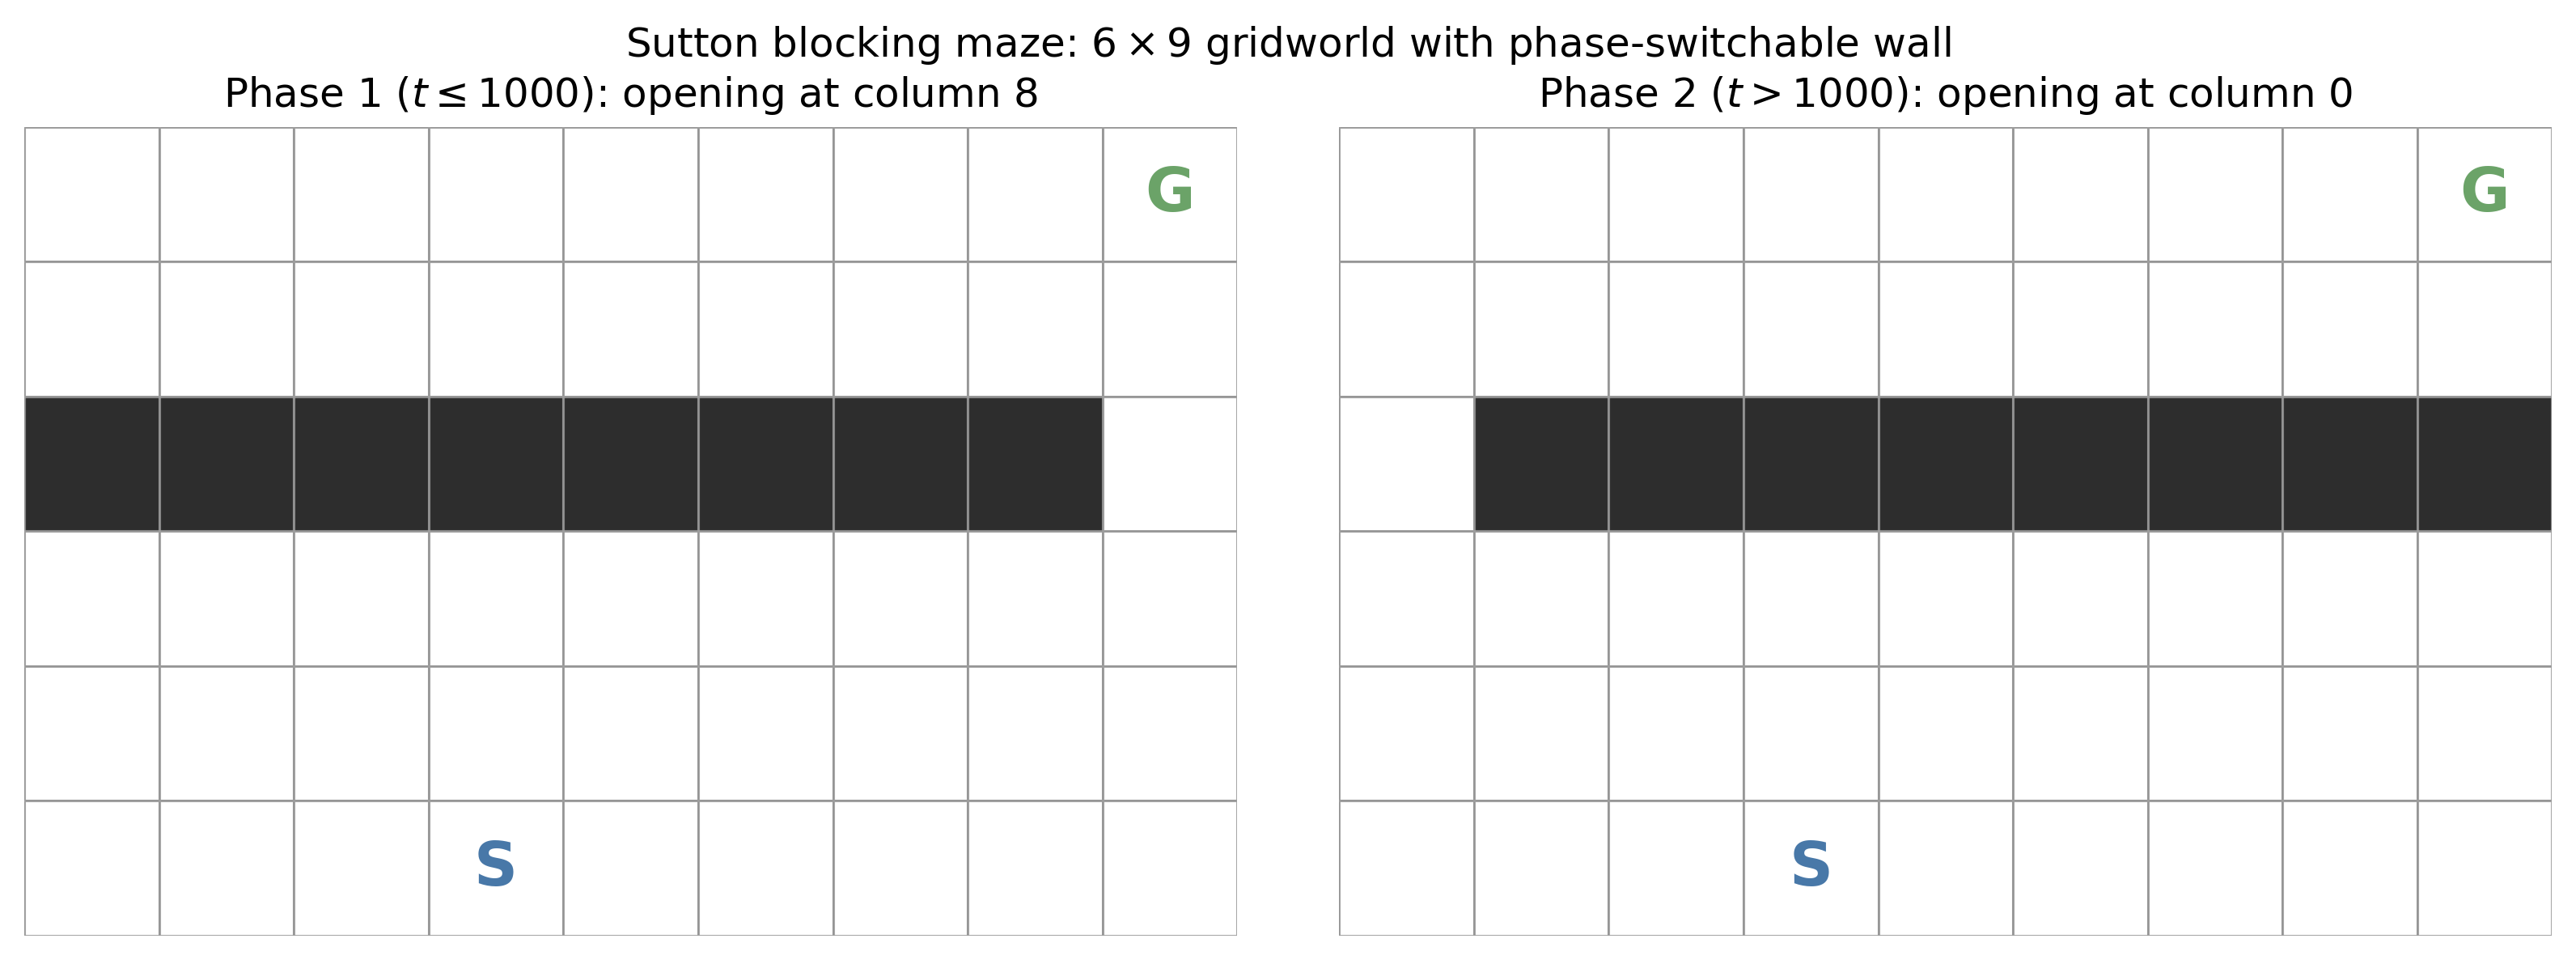
\includegraphics[width=0.95\textwidth]{../ch12_world_models/sims/dyna_maze_layout.png}
  \caption{Sutton blocking maze. The agent starts at $S$ and aims for the goal at $G$; the only opening in the wall along row two shifts from column eight in Phase 1 to column zero in Phase 2 at environment step $t = 1000$. The agent is not notified of the change and observes it only through later transitions.}
  \label{figure:fc_dyna_maze_layout}
\end{figure}

For plain $Q$-learning with $\gamma = 0.95$, $\alpha = 0.1$, $\varepsilon = 0.1$, zero initial $Q$-values, and reward only at the goal, all action values remain tied until the first transition into the goal. Uniform tie-breaking therefore makes action selection uniform before the first positive reward. The expected hitting time of a single random walker from $S$ to $G$ on the open part of this $6 \times 9$ grid is several hundred steps. The first transition into the goal raises one predecessor action value by $\alpha \cdot 1 = 0.1$. Later one-step updates can propagate this value to other state-action pairs. One-step $Q$-learning moves reward information backward only when relevant state-action pairs are revisited. An exploratory action is selected with probability $\varepsilon = 0.1$. Dyna-Q instead samples $K$ state-action pairs from its tabular model after each real interaction, so it can propagate reward information without additional environment steps.

The environment is the $6 \times 9$ deterministic gridworld of \citet{sutton2018}, with start at row five column three and goal at row zero column eight. Actions are the four cardinal moves; transitions are deterministic; the reward is one on goal arrival and zero elsewhere; the discount factor is $\gamma = 0.95$. The wall along row two has its only opening at column eight during Phase 1 ($t \le N_1$ with $N_1 = 1000$) and at column zero during Phase 2 ($N_1 < t \le N_1 + N_2$ with $N_2 = 2000$). The phase flip happens automatically at $t = N_1$ and is not signaled. The total interaction budget is $N_1 + N_2 = 3000$ environment steps, the per-episode step cap is two hundred, and the experiment runs over thirty independent seeds with $\alpha = 0.1$, $\varepsilon = 0.1$, and zero-initialized $Q$.

Five agents share the budget. Plain $Q$-learning with $K = 0$ is the direct-RL baseline, applying only the temporal-difference update of \citet{WatkinsDayan1992} per real step. Dyna-Q with $K = 5$ applies five model-based replays per real step from a tabular Dirac model, and Dyna-Q with $K = 50$ applies fifty; both implement the algorithm box of \S\ref{section:fc_dyna_q_algorithm} with the planning-step count set to the named value.
Dyna-Q+ with $K = 50$ adds the exploration bonus $\kappa \sqrt{\tau(s, a)}$ to planning targets, where $\tau(s, a)$ is the time since the state-action pair was last visited and $\kappa = 10^{-4}$. When a state is encountered, each action not yet tried from that state is added to the model with zero reward and a self-transition. Its elapsed-time bonus then grows until it is tried.
The fifth agent trains a controller with REINFORCE on imagined rollouts from a learned forward model. In \citet{Schmidhuber1990}, the controller is instead updated by analytic gradients propagated through a differentiable model. The agent uses two small multilayer perceptrons. A model network $M_\theta$ maps one-hot state and action vectors to next-state logits and a scalar reward prediction. It is trained on observed transitions using cross-entropy for next state and mean squared error for reward. A controller network $C_\phi$ maps one-hot state to action logits, fit by a REINFORCE policy-gradient estimator on imagined trajectories rolled forward through $M_\theta$. Both networks have a single thirty-two-unit hidden layer. Planning calls happen every ten real steps with sixteen imagined trajectories of length ten and a moving-average baseline. The neural agent and Schmidhuber's 1990 method both use separate model and controller networks, but they differ in network recurrence and in how the controller is updated.

Figure~\ref{figure:fc_dyna_maze} plots mean cumulative environment reward with standard-error bands across thirty seeds. Table~\ref{table:fc_dyna_maze} reports cumulative reward at the end of Phase 1, the reward gained during Phase 2, and total cumulative reward, with rows ordered by total reward at $t = 3000$. At $t = 3000$, mean total rewards are $52.0 \pm 4.2$ for Dyna-Q with $K = 50$, $47.0 \pm 4.4$ for Dyna-Q+ with $K = 50$, $39.2 \pm 4.7$ for Dyna-Q with $K = 5$, $4.0 \pm 0.4$ for the neural controller-model agent, and $3.5 \pm 0.5$ for plain $Q$-learning. Under the equal 3,000-step interaction budget, Dyna-Q with $K = 50$ obtains 14.9 times the mean total reward of $K = 0$. The $K = 50$ agent also performs fifty model-based updates after each real transition, so this comparison does not hold computation fixed. In Phase 1, Dyna-Q+ obtains $37.4 \pm 3.7$ rewards, compared with $42.2 \pm 5.3$ for Dyna-Q. For Dyna-Q+, the implementation adds each untried action to the model with zero reward and a self-transition when its state is encountered, as specified by \citet{sutton2018} in Section~8.3. The neural controller-model agent obtains $4.0 \pm 0.4$ total reward, compared with $3.5 \pm 0.5$ for plain $Q$-learning. Its model and controller are estimated from interaction data, whereas tabular Dyna records each observed transition directly. The experiment does not isolate which difference accounts for the neural agent's result. During Phase 2, Dyna-Q gains $9.8 \pm 4.0$ rewards and Dyna-Q+ gains $9.6 \pm 2.8$. Neither method can correct a transition record affected by the wall change until the corresponding state-action pair is tried again in the environment. A Welch $t$-test of the Phase 2 gains does not reject the null of equal means ($p = 0.968$). The mean total reward for Dyna-Q remains 5.0 higher at $t = 3000$, close to its 4.8-reward Phase 1 difference. Figure~8.4 of \citet{sutton2018} shows earlier recovery for Dyna-Q+ in the blocking maze. The present thirty-seed experiment does not show that separation and does not determine whether a longer post-change budget or a different bonus coefficient would do so. The neural controller-model agent gains $1.5 \pm 0.2$ rewards in Phase 2, compared with $0.6 \pm 0.2$ for plain $Q$-learning. Under this 3,000-step interaction budget, Dyna-Q with $K = 50$ has the highest mean total reward. The experiment does not hold computation fixed and does not test whether the neural controller-model agent becomes more competitive in larger state spaces.

\begin{figure}[ht]
  \centering
  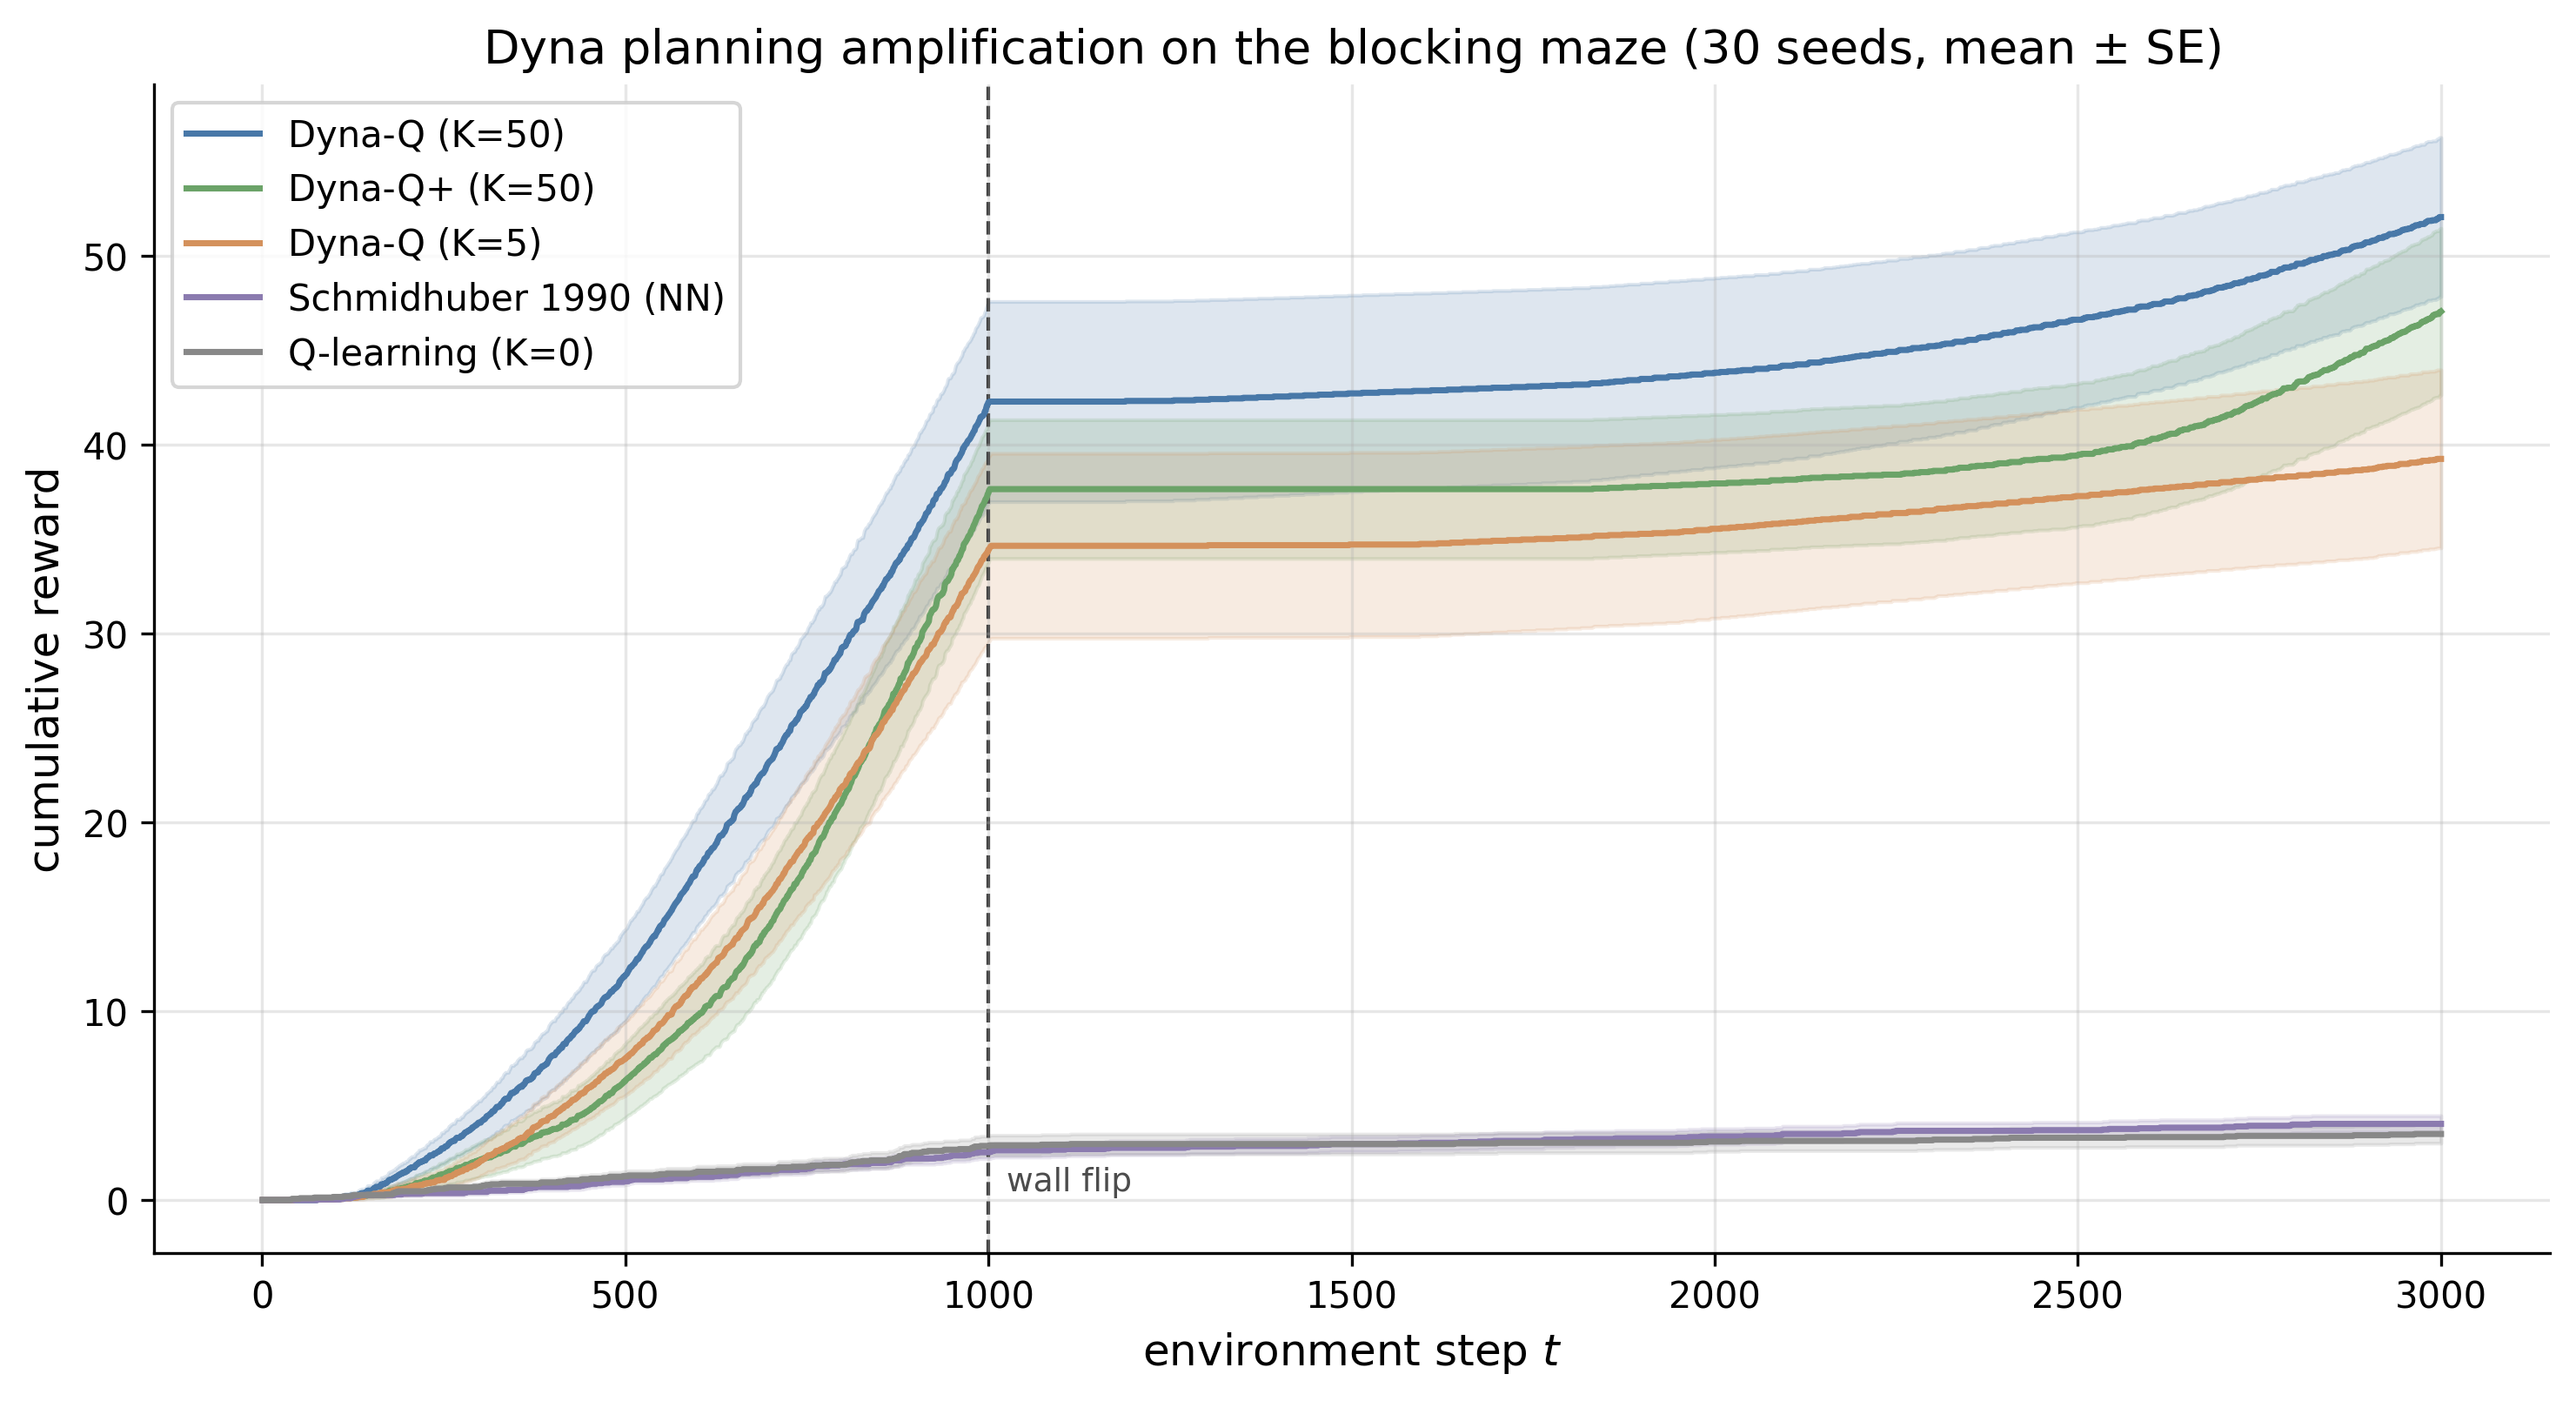
\includegraphics[width=0.95\textwidth]{../ch12_world_models/sims/dyna_maze.png}
  \caption{Cumulative reward on the blocking maze for five agents under a shared three-thousand-step environment budget. The dashed vertical line marks the wall flip at $t = 1000$. Lines are means and shaded bands are one standard error across thirty seeds.}
  \label{figure:fc_dyna_maze}
\end{figure}

\begin{table}[ht]
  \centering
  \caption{Cumulative reward on the blocking maze. End of Phase 1 is at $t = 1000$; Phase 2 gain is the increase over the remaining two thousand steps; Total is the value at $t = 3000$. Mean $\pm$ standard error across thirty seeds.}
  \label{table:fc_dyna_maze}
  % Cumulative reward at end of Phase 1 (t=1000), gain over Phase 2 (last 2000 steps), and total at t=3000.
% Mean +/- SE across 30 seeds.
\begin{tabular}{lrrr}
\toprule
Agent & End of Phase 1 & Phase 2 gain & Total ($t = 3000$) \\
\midrule
Dyna-Q (K=50) & 42.2 $\pm$ 5.3 & 9.8 $\pm$ 4.0 & 52.0 $\pm$ 4.2 \\
Dyna-Q+ (K=50) & 37.4 $\pm$ 3.7 & 9.6 $\pm$ 2.8 & 47.0 $\pm$ 4.4 \\
Dyna-Q (K=5) & 34.4 $\pm$ 4.9 & 4.8 $\pm$ 3.0 & 39.2 $\pm$ 4.7 \\
Schmidhuber 1990 (NN) & 2.5 $\pm$ 0.3 & 1.5 $\pm$ 0.2 & 4.0 $\pm$ 0.4 \\
Q-learning (K=0) & 2.9 $\pm$ 0.5 & 0.6 $\pm$ 0.2 & 3.5 $\pm$ 0.5 \\
\bottomrule
\end{tabular}

\end{table}
